%%%%%%%%%%%%%%%%%%%%%%%%%%%%%%%%%%%%%%%%%%%%%%%%%%%%%%%%%%%%%%%%%%%%%%%%%%%%
%                                                                          %
%   HIGZ  User Guide -- LaTeX Source                                       %
%                                                                          %
%   Chapter: HIGZ examples                                                 %
%                                                                          %
%   Editor: Olivier Couet / CN-AS                                          %
%   Last Mod.:  9 July oc                                                  %
%                                                                          %
%%%%%%%%%%%%%%%%%%%%%%%%%%%%%%%%%%%%%%%%%%%%%%%%%%%%%%%%%%%%%%%%%%%%%%%%%%%%

\chapter{Examples of \HIGZ{} output}

The graphical results of the examples below are reproduced directly 
from the \PS{} output of and introduced into this manual.

\begin{XMPt}{\HIGZ{} test program}
      PROGRAM HIGZEX
*.==========>
*.
*.           HIGZ TEST PROGRAM
*.
*..=========>
      COMMON/PAWC/H(20000)
      LOGICAL INTRAC
      CHARACTER*80 STR
      CHARACTER*(*) HZFILE
+SELF,IF=IBM,IF=-PSCRIPT.
      PARAMETER (HZFILE='/HIGZ METAFILE')
+SELF,IF=IBM,IF=PSCRIPT.
      PARAMETER (HZFILE='/HIGZ PS')
+SELF,IF=-IBM,IF=-PSCRIPT.
      PARAMETER (HZFILE='higz.metafile')
+SELF,IF=-IBM,IF=PSCRIPT.
      PARAMETER (HZFILE='higz.ps')
+SELF.

*.___________________________________________
*
+SELF,IF=IBM.
      CALL ERRSET(151,999,-1)
+SELF,IF=IBM,IF=X11.
      CALL INITC()
+SELF.
      OPEN(10,FILE=HZFILE,FORM='FORMATTED',STATUS='UNKNOWN')
      CALL MZEBRA(-3)
      CALL MZPAW(20000,' ')
      CALL IGINIT(0)
      IF(.NOT.INTRAC(DUMMY))THEN
         INTER=0
         KWTYPE=0
      ELSE
         CALL IGWKTY(KWTYPE)
         INTER=1
      ENDIF
      CALL IGSSE(6,KWTYPE)
      IF(INTER.EQ.0)GOTO 10
      CALL HIEX1
      CALL IRQST(1,1,ISTAT,NCH,STR)
*
*          Switch to alpha mode. Note that IGSSE has preset the
*          workstation identifier to 1
*
      CALL IGSA (1)
*
      PRINT *, ' Example 1 completed'
      CALL HIEX2
      CALL IRQST(1,1,ISTAT,NCH,STR)
      CALL IGSA (1)
      PRINT *, ' Example 2 completed'
*
      CALL HIEX3
      CALL IRQST(1,1,ISTAT,NCH,STR)
      CALL IGSA (1)
      PRINT *, ' Example 3 completed'
*
      CALL HIEX4
      CALL IRQST(1,1,ISTAT,NCH,STR)
      CALL IGSA (1)
      PRINT *, ' Example 4 completed'
*
  10  CALL HIEX5
      IF(INTER.EQ.0)GOTO 20
      CALL IGSA (1)
      PRINT *, ' Example 5 completed'
*
*          Replay some pictures from the HIGZ metafile
*
      CALL HIEX6
      CALL IGSA (1)
      PRINT *, ' Example 6 completed'
*
  20  CALL IGEND
      END
\end{XMPt}

\newpage
\begin{XMPt}{Example of basic HIGZ. Polylines and fill areas}
\label{HIEX1}
      SUBROUTINE HIEX1
*
      COMMON /QUEST/ RQUEST(100)
      DIMENSION XZ(86),YZ(86)
      DATA XZ/
     +   0.6250,0.6875,0.9063,0.7500,0.7500,0.6875,0.6250,0.6875
     +  ,0.7500,0.8750,0.9688,1.0313,1.1563,1.2500,1.3125,1.5000
     +  ,1.6875,1.9375,2.0000,2.1250,2.1875,2.1875,2.2500,2.2500
     +  ,2.4375,2.4375,2.4688,2.5313,2.5313,2.5000,2.6250,2.6250
     +  ,2.7500,2.7188,2.7188,2.7188,2.9375,3.4375,3.7500,4.0625
     +  ,4.1250,4.0625,4.1250,4.1875,4.3125,4.3125,4.3125,4.3438
     +  ,4.3125,4.4375,4.5000,4.4375,4.4375,4.5625,4.5938,4.7188
     +  ,4.7813,4.7500,4.5313,4.5000,4.6250,4.6875,4.7188,4.7500
     +  ,4.8750,4.9625,4.9063,4.7500,4.6875,4.6563,4.3750,3.6875
     +  ,3.0625,2.8125,2.4375,2.0313,1.6563,1.4688,1.3438,1.3750
     +  ,1.4375,1.2500,1.1250,1.0000,0.8750,0.6250/
      DATA YZ/
     +   4.8750,4.6563,4.3750,4.1250,3.8750,3.6250,3.4375,3.3125
     +  ,3.1875,3.1563,3.2188,3.3438,3.5000,3.5938,3.6875,3.5625
     +  ,3.3125,3.0938,2.8438,2.7000,2.2188,1.8750,1.2813,1.0625
     +  ,1.0625,1.8750,2.5000,2.4688,2.1875,1.9688,1.5000,1.2500
     +  ,1.2500,1.5313,2.0625,2.6250,2.5938,2.6563,2.7500,3.0000
     +  ,2.7188,2.1250,1.6563,1.4375,1.4688,1.6250,2.0313,2.3125
     +  ,2.6250,2.3125,2.0625,1.6250,1.5000,1.5000,1.6250,2.0313
     +  ,2.3125,2.5000,2.7500,2.9375,3.2500,3.6250,3.2500,2.8125
     +  ,2.6250,2.6875,3.0625,3.5625,3.8750,4.0625,4.1875,4.1250
     +  ,4.0313,4.0938,4.0625,4.2500,4.4875,4.5000,4.4688,4.6875
     +  ,4.8750,4.7188,4.5250,4.4688,4.7188,4.8750/
      DATA NZ/86/
*
*          Define the size of the Picture in cm
*
      CALL ICLRWK(0,1)
      CALL IGRNG(14.5,14.5)
      R  = RQUEST(11)
      XL = RQUEST(12)
      YB = RQUEST(13)
      CALL IGBOX(0.,14.5,0.,14.5)
      CALL IGTEXT(7.25,13.5,'HIGZ example 1',0.6,0.,'C')
*
*          Define a new Normalization transformation for each new object
*          The viewports are set in the centimeter space defined by IGRNG
*
      CALL ISWN(10,0.,5.,0.,5.)
      CALL ISVP(10,0.5*R+XL,6.5*r+XL,6.5*R+YB,11.5*r+YB)
      CALL ISELNT(10)
      CALL IPL(NZ,XZ,YZ)
*
      CALL ISWN(20,0.,5.,0.,5.)
      CALL ISVP(20,7.5*R+XL,14.*r+XL,6.5*R+YB,11.5*r+YB)
      CALL ISELNT(20)
      CALL ISMK(29)
      CALL IPM(NZ-1,XZ,YZ)
      CALL IPL(NZ  ,XZ,YZ)
*
      CALL ISWN(30,0.,5.,0.,5.)
      CALL ISVP(30,0.5*R+XL,6.5*r+XL,0.5*R+YB,5.5*r+YB)
      CALL ISELNT(30)
      CALL ISFAIS(3)
      CALL ISFASI(256)
      CALL IFA(NZ-1,XZ,YZ)
*
      CALL ISWN(40,0.,5.,0.,5.)
      CALL ISVP(40,7.5*R+XL,14.*r+XL,0.5*R+YB,5.5*r+YB)
      CALL ISELNT(40)
      CALL ISFASI(290)
      CALL IFA(NZ-1,XZ,YZ)
      CALL ISFAIS(0)
      CALL IFA(NZ-1,XZ,YZ)
*
      END
\end{XMPt}
\newpage

\begin{minipage}{\textwidth}
\begin{Fighere}
\begin{center}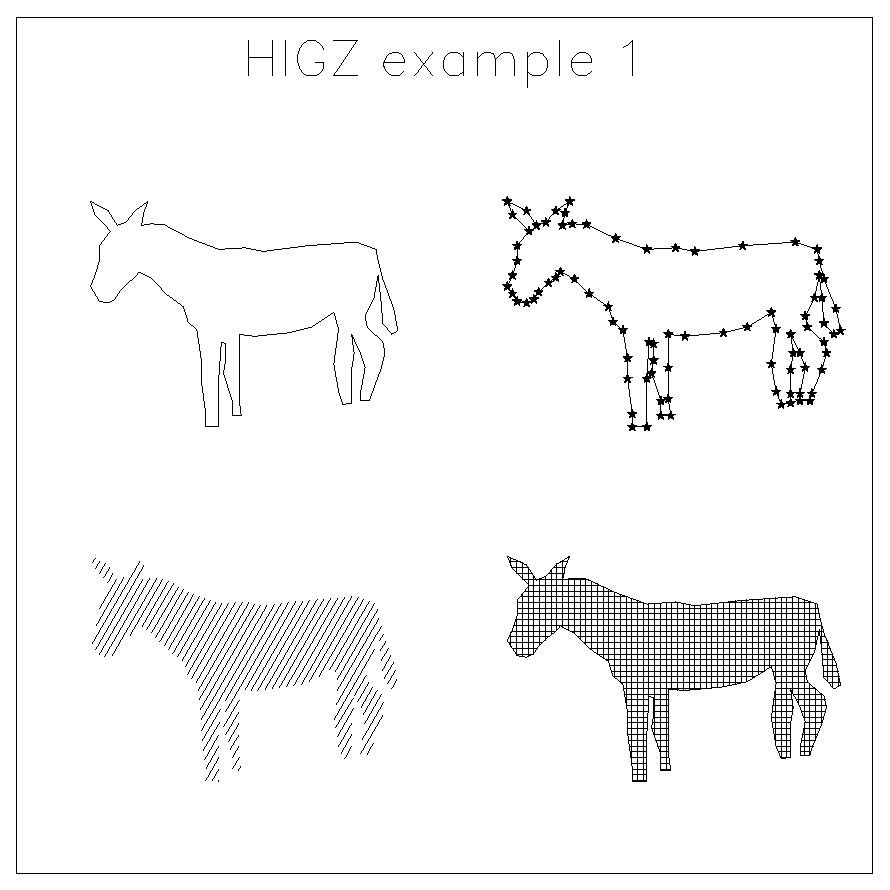
\includegraphics{higz1.eps}\end{center}
\caption{Result of first \protect\HIGZ{} example}
\end{Fighere}
\end{minipage}

\newpage

\begin{XMPt}{Example to plot the table of \HIGZ{} software characters}
      SUBROUTINE HIEX2
*
      CHARACTER*6 KD1,KD2
      CHARACTER*45 KDG
      CHARACTER*3 KTEXT
      CHARACTER*1 CHOPT
      DIMENSION XPOS(6),X(5),Y(5)
      DATA KD1/' < < <'/
      DATA KD2/'  [[""'/
      DATA KDG/'ABCDEFGHIJKLMNOPQRSTUVWXYZ0123456789.,+-*/=()'/
      DATA XLONG,YTOP/16.,24./
      DATA SIZE,ANGLE/0.3,0./
*
      CALL IGRNG(20.,24.)
      CALL ICLRWK(0,1)
*
      XW = XLONG/12.
      DO 10 I = 1,6
         XPOS(I) = (2*I-1)*XW + 2.5
  10  CONTINUE
*
*              Draw the frame
*
      YLONG  = 46*1.5*SIZE + 5*1.5*SIZE
      X(1)   = XPOS(1) - XW
      X(2)   = XPOS(6) + XW
      X(3)   = X(2)
      X(4)   = X(1)
      X(5)   = X(1)
      Y(1)   = YTOP
      Y(2)   = Y(1)
      Y(3)   = Y(1) - YLONG
      Y(4)   = Y(3)
      Y(5)   = Y(1)
      CALL IPL(5,X,Y)
      DO 20 I = 1,5
         X(1)   = XPOS(I) + XW
         X(2)   = X(1)
         Y(1)   = YTOP
         Y(2)   = Y(1) - YLONG
         CALL IPL(2,X,Y)
  20  CONTINUE
      X(1)   = XPOS(1) - XW
      X(2)   = XPOS(6) + XW
      Y(1)   = YTOP - 5.*SIZE
      Y(2)   = Y(1)
      CALL IPL(2,X,Y)
*
*             Draw box titles
*
      Y1     = YTOP - 2.*SIZE
      Y2     = Y1 - 2.*SIZE
      CHOPT='C'
      CALL IGTEXT(XPOS(1),Y1,'Upper'  ,SIZE,ANGLE,CHOPT)
      CALL IGTEXT(XPOS(1),Y2,'Roman'  ,SIZE,ANGLE,CHOPT)
      CALL IGTEXT(XPOS(2),Y1,'Lower'  ,SIZE,ANGLE,CHOPT)
      CALL IGTEXT(XPOS(2),Y2,'Roman'  ,SIZE,ANGLE,CHOPT)
      CALL IGTEXT(XPOS(3),Y1,'Upper'  ,SIZE,ANGLE,CHOPT)
      CALL IGTEXT(XPOS(3),Y2,'Greek'  ,SIZE,ANGLE,CHOPT)
      CALL IGTEXT(XPOS(4),Y1,'L<OWER' ,SIZE,ANGLE,CHOPT)
      CALL IGTEXT(XPOS(4),Y2,'G<REEK' ,SIZE,ANGLE,CHOPT)
      CALL IGTEXT(XPOS(5),Y1,'U<PPER' ,SIZE,ANGLE,CHOPT)
      CALL IGTEXT(XPOS(5),Y2,'Special',SIZE,ANGLE,CHOPT)
      CALL IGTEXT(XPOS(6),Y1,'Lower'  ,SIZE,ANGLE,CHOPT)
      CALL IGTEXT(XPOS(6),Y2,'Special',SIZE,ANGLE,CHOPT)
*
      YP = YTOP - 6.*SIZE
      DO 40 I = 1,45
         YP = YP - 1.5*SIZE
         DO 30 J = 1,6
            KTEXT=KD1(J:J)//KD2(J:J)//KDG(I:I)
            CALL IGTEXT(XPOS(J),YP,KTEXT,SIZE,ANGLE,CHOPT)
  30     CONTINUE
  40  CONTINUE
*
      END
\end{XMPt}

\begin{figure}[p]
\begin{center}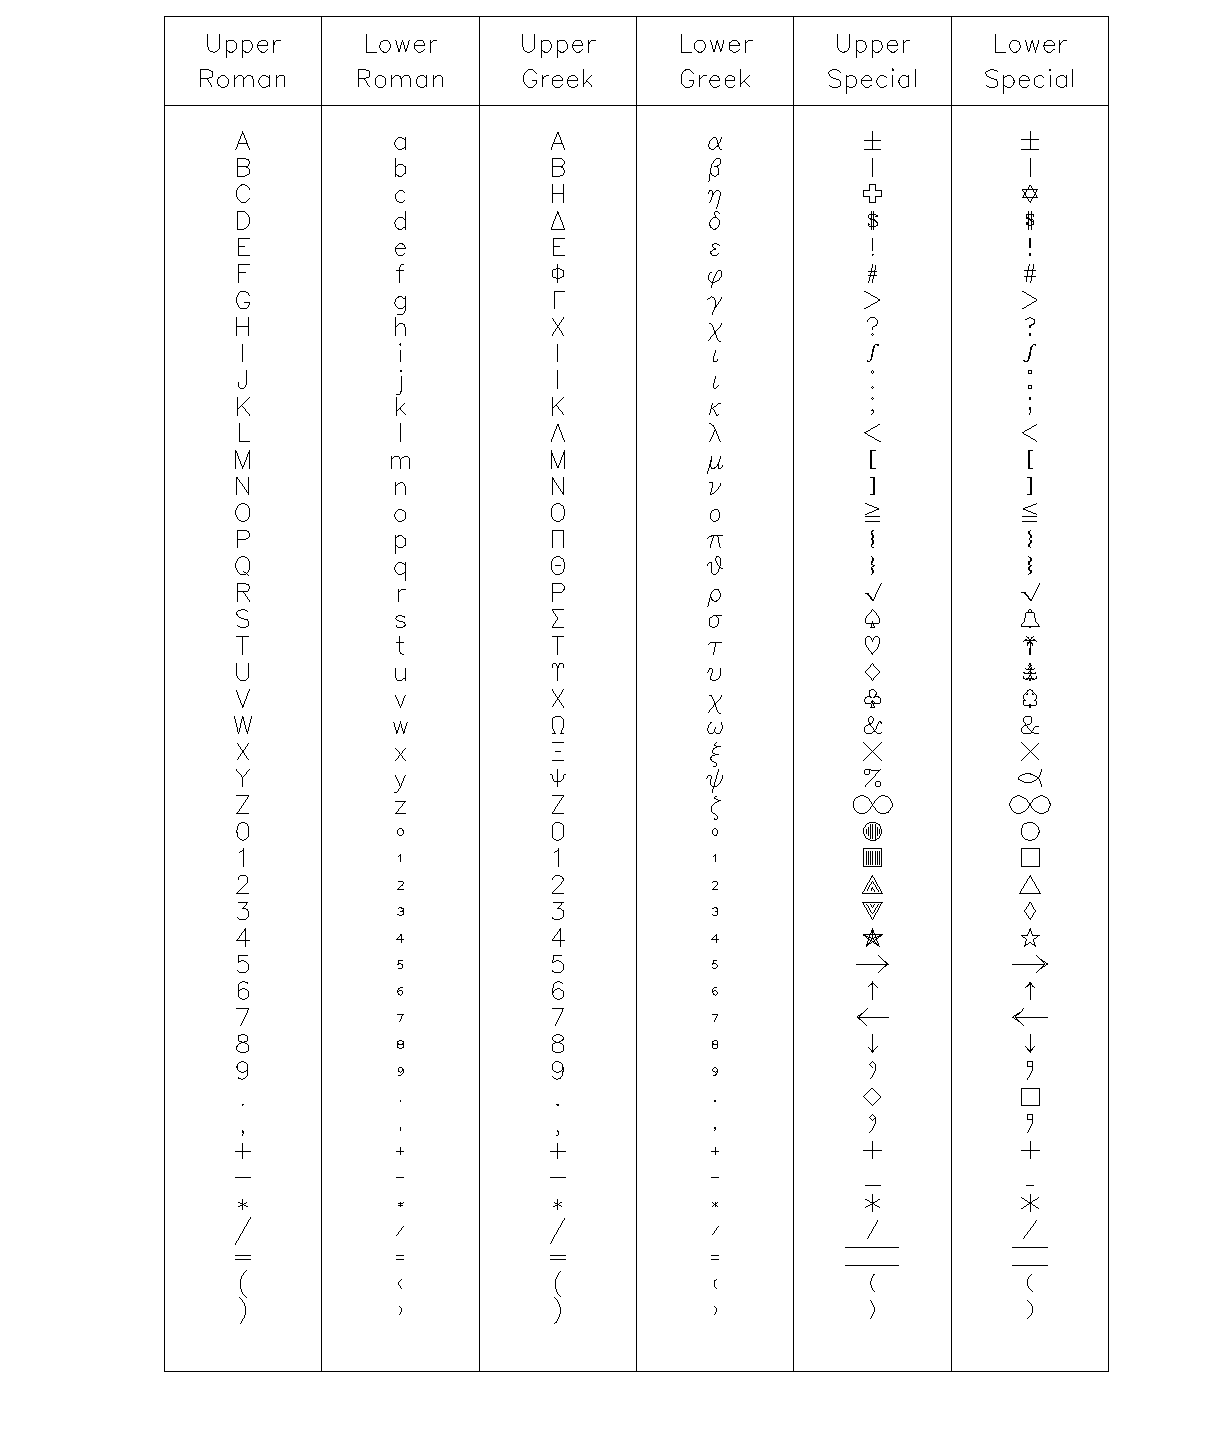
\includegraphics[width=\linewidth]{higz2.eps}\end{center}
\caption{Result of plotting \protect\HIGZ{} software characters}
\end{figure}
\clearpage

\begin{XMPt}{Advanced example to draw text (based on a PAW macro from W.Walk)}
      SUBROUTINE HIEX3
*
      DIMENSION X(3),Y(3)
*
      CALL IGRNG(14.6,18.)
      CALL ICLRWK(0,1)
      CALL IGBOX(0.,14.6,0.,18.)
      CALL IGSET('PASS',10.)
      CALL IGSET('CSHI',0.005)
      CALL ISFAIS(1)
      CALL ISTXCI(1)
      CALL ISTXFP(-104,2)
      CALL ISCHH(0.6)
      CALL ISTXAL(2,0)
      CALL ITX(7.3,17.,'Exclusive Toponium Decays')
      CALL ISTXFP(0,2)
      CALL ISFACI(1)
      CALL IGBOX(5.,7.,15.,14.9)
      CALL IGBOX(5.,7.,3.,2.9)
      CALL IGBOX(3.,5.,14.,13.9)
      CALL IGBOX(3.,5.,2.,1.9)
      CALL IGBOX(10.,12.,13.,12.9)
      CALL IGBOX(10.,12.,12.,11.9)
      CALL IGBOX(10.,12.,11.,10.9)
      CALL IGBOX(6.,8.,12.4,12.3)
      CALL ISPLCI(3)
      X(1)=6.
      X(2)=11.
      X(3)=6.
      Y(1)=15.
      Y(2)=13.
      Y(3)=3.
      CALL IPL(3,X,Y)
      Y(2)=12.
      CALL IPL(3,X,Y)
      Y(2)=11.
      CALL IPL(3,X,Y)
      CALL ISPLCI(2)
      X(2)=4.
      Y(2)=14.
      CALL IPL(3,X,Y)
      Y(2)=2.
      CALL IPL(3,X,Y)
      CALL ISPLCI(4)
      X(2)=X(3)
      Y(2)=1.5
      CALL IPL(2,X(2),Y(2))
      X(1)=X(2)-0.2
      X(3)=X(2)+0.2
      Y(1)=Y(2)+0.3
      Y(3)=Y(1)
      CALL IPL(3,X,Y)
      CALL ISTXCI(4)
      CALL IGTEXT(6.,0.5,'e^+!e^-! or [m]^+![m]^-!',0.5,0.,'C')
      CALL IGTEXT(6.,15.2,'2^3!S?1--!',0.5,0.,'C')
      CALL IGTEXT(6.,3.2,'1^3!S?1--!',0.5,0.,'C')
      CALL IGTEXT(11.,13.2,'1^3!P?2++!',0.5,0.,'C')
      CALL IGTEXT(11.,12.2,'1^3!P?1++!',0.5,0.,'C')
      CALL IGTEXT(11.,11.2,'1^3!P?0++!',0.5,0.,'C')
      CALL IGTEXT(7.,12.6,'1^1!P?1+-!',0.5,0.,'C')
      CALL IGTEXT(4.,14.2,'2^1!S?0-+!',0.5,0.,'C')
      CALL IGTEXT(4., 2.2,'1^1!S?0-+!',0.5,0.,'C')
      CALL ISTXCI(6)
      CALL IGTEXT(4.5,15.,'[Q]?2S!',0.5,0.,'R')
      CALL IGTEXT(7.5,2.75,'[Q]?1S! (80 GeV)',0.5,0.,'L')
      CALL IGTEXT(2.5,13.75,'[c]?t!&^,!',0.5,0.,'R')
      CALL IGTEXT(2.5,1.75,'[c]?t!',0.5,0.,'R')
      CALL IGTEXT(12.5,13.,'[h]^2!&?t!',0.5,0.,'L')
      CALL IGTEXT(12.5,12.,'[h]^1!&?t!',0.5,0.,'L')
      CALL IGTEXT(12.5,11.,'[h]^0!&?t!',0.5,0.,'L')
      CALL ISTXCI(3)
      CALL IGTEXT(1.,9.,'E1',0.5,0.,'C')
      CALL ISTXCI(2)
      CALL IGTEXT(3.,9.,'M1',0.5,0.,'C')
      CALL ISTXCI(3)
      CALL IGTEXT(8.8,14.8,'100 MeV',0.4,0.,'L')
      CALL IGTEXT(8.5,6.,'800 MeV',0.4,0.,'L')
      CALL ISTXCI(6)
      CALL IGTEXT(9.4,14.2,'BR 2"Y',0.3,0.,'L')
      CALL IGTEXT(8.9,5.4,'BR 30"Y',0.3,0.,'L')
      CALL IGSET('*',0.)
*
      END
\end{XMPt}

\begin{figure}[p]
\begin{center}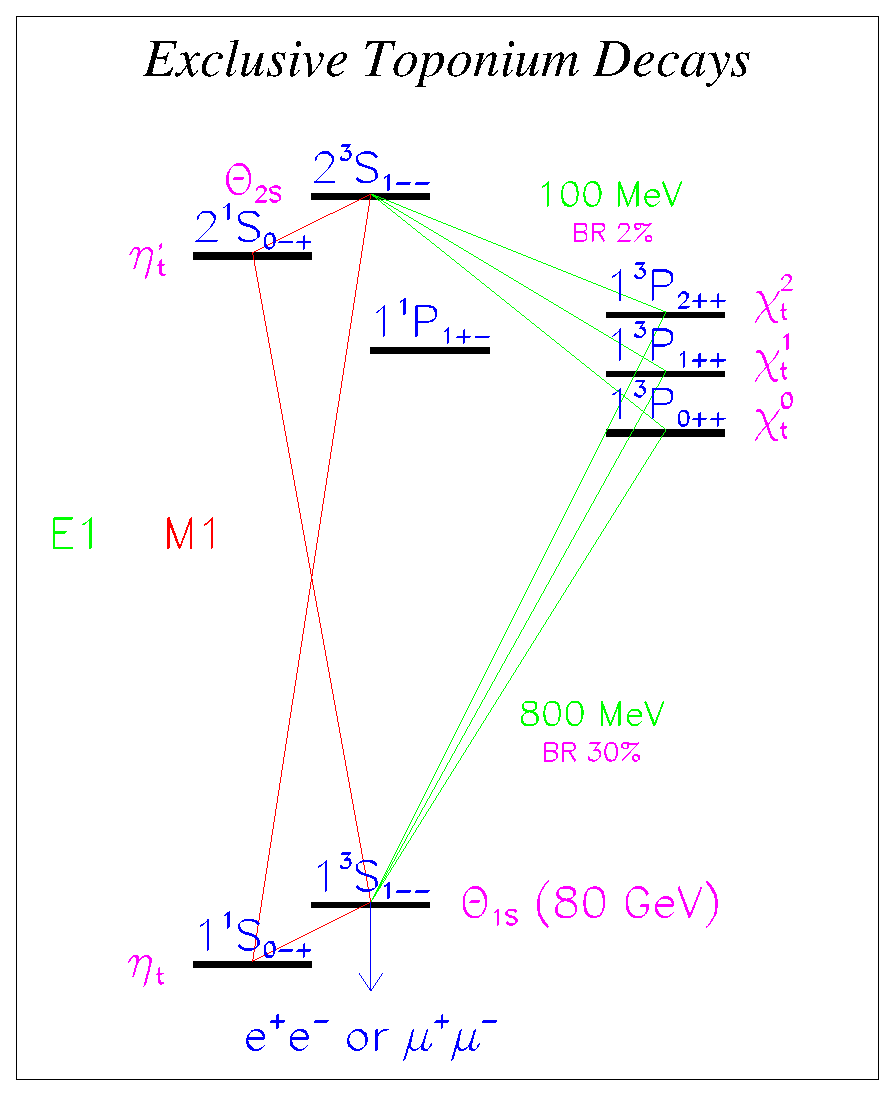
\includegraphics{higz3.eps}\end{center}
\caption{Result of \protect\HIGZ{} example 3 (toponium decay scheme)}
\end{figure}
\clearpage

\begin{XMPt}{Examples of graphs and histograms}
\label{HIEX4}
      SUBROUTINE HIEX4
*
      COMMON /QUEST/ RQUEST(100)
      DIMENSION X(10),Y(10),V(10)
      DATA Y/2.,3.,5.,4.,7.,10.,11.,9.,10.,4./
      DATA X/0.,16.,8*0./
      DATA V/-1.5,1.,2.,4.,4.5,6.,9.,10.,14.,17./
*
      CALL IGRNG(15.,18.)
      R  = RQUEST(11)
      XL = RQUEST(12)
      YB = RQUEST(13)
      CALL ICLRWK(0,1)
      CALL ISTXFP(-13,1)
*
      CALL ISWN(10,0.,18.,-1.,12.)
      CALL ISVP(10,8.*R+XL,14.*R+XL,11.*R+YB,17.*R+YB)
      CALL ISELNT(10)
      CALL ISMK(29)
      CALL IGHIST(10,X,Y,'AHCP')
*
      CALL ISWN(20,0.,18.,0.,12.)
      CALL ISVP(20,R+XL,7.*R+XL,11.*R+YB,17.*R+YB)
      CALL ISELNT(20)
      CALL IGHIST(10,X,Y,'AB')
*
      CALL ISWN(30,-4.,19.,-1.,13.)
      CALL ISVP(30,R+XL,14.*R+XL,R+YB,10.*R+YB)
      CALL ISELNT(30)
      CALL IGAXIS(-3.,19.,1.,1.,-3.,19.,20510,' ')
      CALL IGSET('LASI',0.5)
      CALL IGAXIS(-3.,-3.,1.,12.,1.,12.,510,'H')
      CALL ISMK(21)
      CALL IGRAPH(10,V,Y,'LP')
      CALL ISLN(2)
      CALL IGRAPH(10,V,Y,'C')
      CALL IGSET('*',0.)
*
      END
\end{XMPt}

\begin{figure}[p]
\begin{center}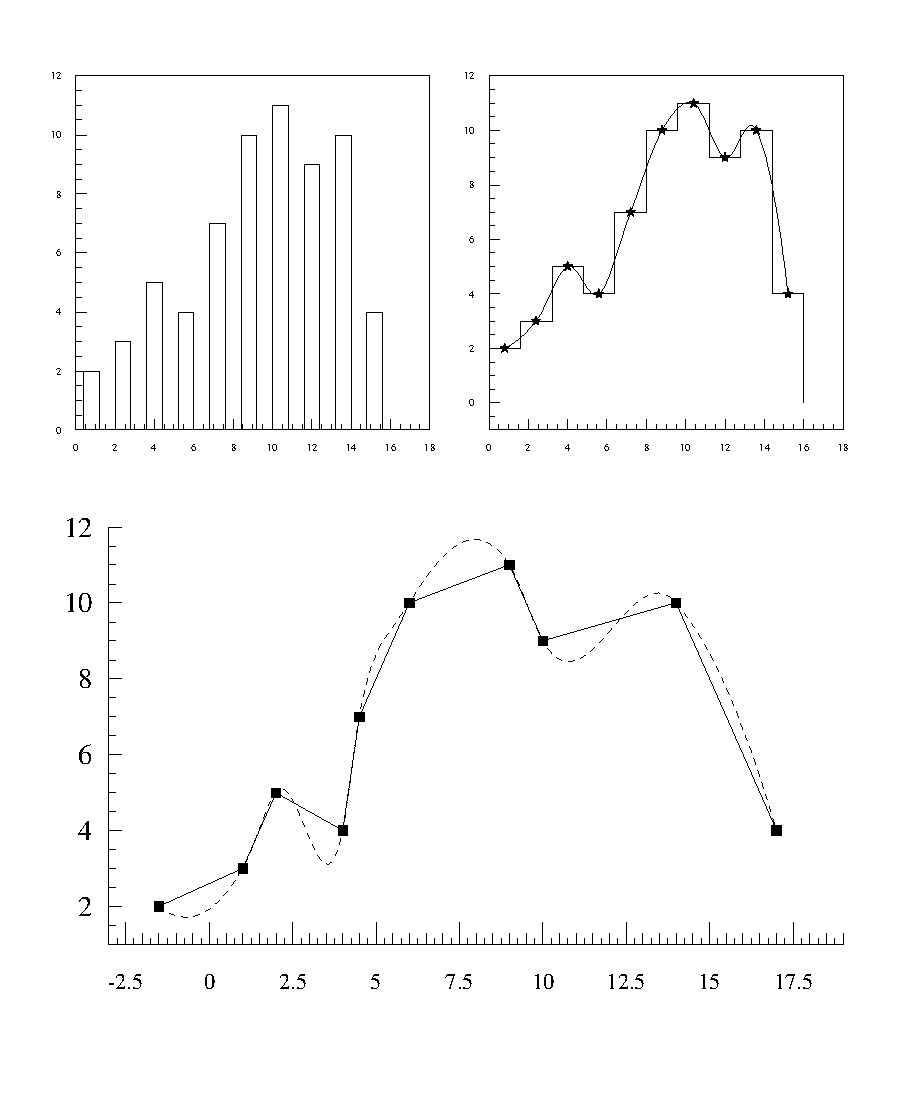
\includegraphics{higz4.eps}\end{center}
\caption{Result of \protect\HIGZ{} example 4 (graphs and histograms)}
\end{figure}
\clearpage

\begin{XMPt}{Example using \HIGZ{} and \PS{} metafiles}
      SUBROUTINE HIEX5
*
*          Open HIGZ metafile
*          and repeat previous examples
*
      PRINT *,' Writing higz metafile'
      CALL IGZSET('Z')
      CALL IZOPEN(1,'Pictures','higz.rz','AN',1024,ISTAT)
      CALL IZPICT('ZEBRA','M')
      CALL HIEX1
      CALL IZPICT('SOFT-TABLE','M')
      CALL HIEX2
      CALL IZPICT('TOPONIUM','M')
      CALL HIEX3
      CALL IZPICT('GRAPH','M')
      CALL HIEX4
      CALL IZOUT('GRAPH',ICYCLE)
      CALL IGSA (1)
*
*          Open PostScript metafile
*          and repeat previous examples
*
      PRINT *,' Writing PostScript metafile'
      CALL IGZSET('G')
      CALL IGMETA(-10,0)
      CALL HIEX1
      CALL HIEX2
      CALL HIEX3
      CALL HIEX4
      CALL IGMETA(0,0)
*
      END
\end{XMPt}

\newpage

\begin{XMPt}{Display pictures in \HIGZ{} files and invoke the \HIGZ{} editor}
      SUBROUTINE HIEX6
*
      CHARACTER*10 STR
      DATA ICYCLE/999/
*
*           List contents of the ZEBRA/RZ file
*
      CALL RZLDIR(' ',' ')
*
*           Read some pictures into memory and display
*
      CALL IGSET('AURZ',0.)
      CALL IZIN('ZEBRA',ICYCLE)
      CALL IZPICT('ZEBRA','D')
      CALL IRQST(1,1,ISTAT,NCH,STR)
      CALL IZIN('TOPONIUM',ICYCLE)
      CALL IZPICT('TOPONIUM','D')
      CALL IRQST(1,1,ISTAT,NCH,STR)
*
*           Edit PICT4
*           Select options in the graphics menu
*           For example select the item ARROW in the
*           menu 'PRIMITIVES', select the type of arrow
*           by clicking in the box 'ATTR' and try to superimpose
*           a double-arrow on the picture.
*           Try to change the font and the font size for the top graphs
*           Note that the HIGZ graphics editor can be invoked
*           from PAW (PICTURE/MODIFY command).
*
      CALL IZGED('GRAPH',' ')
*
      END
\end{XMPt}
